% Cartel repeated-game decision tree (A6).
\documentclass[border=10pt,tikz]{standalone}
\usepackage{tikz}
\usetikzlibrary{arrows.meta,positioning,fit,calc,decorations.pathmorphing}

\definecolor{sand}{HTML}{E9DCC4}
\definecolor{sanddeep}{HTML}{D4C5A9}
\definecolor{ebony}{HTML}{1E1B18}
\definecolor{ink}{HTML}{2C2A26}
\definecolor{cinnabar}{HTML}{CC3D2E}
\definecolor{brass}{HTML}{B08D57}
\definecolor{patina}{HTML}{5C7A6A}
\definecolor{paper}{HTML}{FBF7EE}

\begin{document}
\begin{tikzpicture}[
  font=\sffamily\small,
  state/.style={draw=ebony,thick,fill=sand,circle,inner sep=2pt,
                minimum size=9mm,font=\sffamily\footnotesize},
  decision/.style={draw=ebony,thick,fill=paper,rounded corners=3pt,
                   inner sep=4pt,align=center,minimum width=22mm},
  payoff/.style={draw=patina,thick,fill=paper,rounded corners=2pt,
                 inner sep=3pt,align=center,
                 font=\sffamily\footnotesize\bfseries},
  bad/.style={draw=cinnabar,thick,fill=paper,rounded corners=2pt,
              inner sep=3pt,align=center,
              font=\sffamily\footnotesize\bfseries,text=cinnabar},
  arr/.style={->,>=Latex,thick,draw=ink},
  prob/.style={font=\sffamily\footnotesize\itshape,fill=paper,inner sep=1pt},
]

\node[font=\sffamily\bfseries,anchor=west] at (-0.4,4.6)
  {Cartel repeated-game node (per round): grim-trigger strategy};

% Round t state.
\node[state] (rt) at (0,2.8) {round $t$};

% Decision: collude vs defect
\node[decision,right=12mm of rt] (dec) {Action choice};
\draw[arr] (rt) -- (dec);

% Collude branch
\node[decision,fill=patina!30,right=14mm of dec,yshift=18mm] (collude)
  {COLLUDE\\charge $q_{\mathrm{floor}}$};
\draw[arr] (dec.north east) to[bend left=10] (collude.west);

% Defect branch
\node[decision,fill=brass!40,right=14mm of dec,yshift=-18mm] (defect)
  {DEFECT\\undercut by $\varepsilon$};
\draw[arr] (dec.south east) to[bend right=10] (defect.west);

% From COLLUDE: detected vs not
\node[state,right=18mm of collude,yshift=12mm] (det)
  {detected};
\node[state,right=18mm of collude,yshift=-12mm] (safe)
  {survived};
\draw[arr] (collude.east) to[bend left=10]
  node[prob,above]
  {$p_d$} (det.west);
\draw[arr] (collude.east) to[bend right=10]
  node[prob,below]
  {$1-p_d$} (safe.west);

% Payoffs
\node[bad,right=4mm of det] {$-5(q_f - \mu)$\\(slash)};
\node[payoff,right=4mm of safe] {$+\pi_C$\\(continue)};

% From DEFECT: one-shot then collapse
\node[state,right=18mm of defect] (collapse) {collapse};
\draw[arr] (defect.east) -- (collapse.west);
\node[payoff,right=4mm of collapse,fill=brass!20]
  {$+\pi_D$ once,\\then $\pi_N \approx 0$};

% Sustainability condition
\node[draw=ebony,thick,fill=sanddeep,rounded corners=3pt,
      align=left,inner sep=6pt,
      below=14mm of dec,minimum width=110mm]
  (cond)
  {{\bfseries Folk-theorem sustainability (one-shot-deviation principle):}
   \\[2pt]
   $\dfrac{\delta \cdot \pi_C}{1 - \delta(1 - p_d)} \;\geq\; \pi_D$
   \quad $\Leftrightarrow$ \quad
   $p_d^\star \;=\; 1 - \dfrac{\pi_C - (1 - \delta)\pi_D}{\delta \cdot \pi_D}$};

% Empirical threshold callout
\node[draw=cinnabar,thick,fill=paper,rounded corners=2pt,inner sep=4pt,
      below=4mm of cond,align=left,minimum width=80mm]
  {{\bfseries Empirical (sim):} at $\delta=0.95$, $p_d^\star \approx 0.10$.\\
   Protocol must achieve $\geq 10\%$ per-round detection to break cartels.};

\end{tikzpicture}
\end{document}
